\begin{frame}{Work-stealing}
\centering
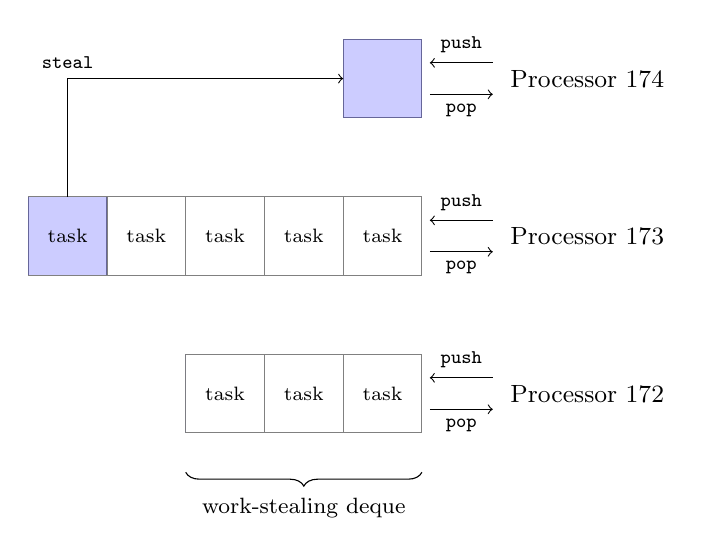
\begin{tikzpicture}
	\def\sep{1}
	\def\hsep{0.1}
	\def\vsep{0.3}
	\def\lenI{3}
	\def\lenxI{0}
	\def\lenII{4}
	\def\lenxII{1}
	\def\lenIII{0}
	\def\lenxIII{1}
	
	\node[right] at (1, 0.5) {\small Processor \ding{172}} ;
	\draw[step=1cm, gray] (0, 0) grid ++(-\lenI, 1) ;
	\draw[step=1cm, gray] (-\lenI, 0) grid ++(-\lenxI, 1) ;
	\fill[blue, opacity=0.2] (-\lenI, 0) rectangle ++(-\lenxI, 1) ;
	\draw[decorate, decoration={brace, amplitude=5pt}] (0, -0.5) -- ++(-\lenI, 0) node [midway, below, yshift=-2mm] {\footnotesize work-stealing deque} ;
	\draw[->] (\hsep, \vsep) -- ++(1 - 2 * \hsep, 0) node[midway, below] {\scriptsize\texttt{pop}} ;
	\draw[->] (1 - \hsep, 1 - \vsep) -- ++(2 * \hsep - 1, 0) node[midway, above] {\scriptsize\texttt{push}} ;
	\foreach \x in {1, ..., \lenI} {
		\node at (0.5 - \x, 0.5) {\scriptsize task} ;
	}
	
	\node[right] at (1, \sep + 1.5) {\small Processor \ding{173}} ;
	\draw[step=1cm, gray] (0, \sep + 1) grid ++(-\lenII, 1) ;
	\draw[step=1cm, gray] (-\lenII, \sep + 1) grid ++(-\lenxII, 1) ;
	\fill[blue, opacity=0.2] (-\lenII, \sep + 1) rectangle ++(-\lenxII, 1) ;
	\draw[->] (\hsep, \sep + 1 + \vsep) -- ++(1 - 2 * \hsep, 0) node[midway, below] {\scriptsize\texttt{pop}} ;
	\draw[->] (1 - \hsep, \sep + 2 - \vsep) -- ++(2 * \hsep - 1, 0) node[midway, above] {\scriptsize\texttt{push}} ;
	\foreach \x in {1, ..., \lenII} {
		\node at (0.5 - \x, \sep + 1.5) {\scriptsize task} ;
	}
	\node at (0.5 - \lenII - \lenxII, \sep + 1.5) {\scriptsize task} ;
	
	\node[right] at (1, 2 * \sep + 2.5) {\small Processor \ding{174}} ;
	\draw[step=1cm, gray] (0, 2 * \sep + 2) grid ++(-\lenIII, 1) ;
	\draw[step=1cm, gray] (-\lenIII, 2 * \sep + 2) grid ++(-\lenxIII, 1) ;
	\fill[blue, opacity=0.2] (-\lenIII, 2 * \sep + 2) rectangle ++(-\lenxIII, 1) ;
	\draw[->] (\hsep, 2 * \sep + 2 + \vsep) -- ++(1 - 2 * \hsep, 0) node[midway, below] {\scriptsize\texttt{pop}} ;
	\draw[->] (1 - \hsep, 2 * \sep + 3 - \vsep) -- ++(2 * \hsep - 1, 0) node[midway, above] {\scriptsize\texttt{push}} ;
	
	\draw[->, to path={|- node[above] {\scriptsize\texttt{steal}} (\tikztotarget)}] (0.5 - \lenII - \lenxII, \sep + 2) to (- \lenIII - \lenxIII, 2 * \sep + 2.5) ;
\end{tikzpicture}
\end{frame}

% ---------------------------------------------------------

\begin{frame}{Chase-Lev work-stealing deque}
\begin{enumerate}
	\item
		\textit{The Implementation of the Cilk-5 Multithreaded Language}. \\
		Frigo, Leiserson \& Randall (1998).
		\begin{itemize}
			\item lock
		\end{itemize}
	\item
		\textit{Thread Scheduling for Multiprogrammed Multiprocessors}. \\
		Arora, Blumofe \& Plaxton (1998).
		\begin{itemize}
			\item non-blocking
			\item one fixed size array, potential overflow
		\end{itemize}
	\item
		\textit{A dynamic-sized nonblocking work stealing deque}. \\
		Hendler, Lev, Moir \& Shavit (2004).
		\begin{itemize}
			\item non-blocking
			\item list of small arrays, no overflow
		\end{itemize}
	\item
		\underline{\textit{Dynamic circular work-stealing deque}}. \\
		Chase \& Lev (2005).
		\begin{itemize}
			\item non-blocking
			\item circular arrays, no overflow
		\end{itemize}
\end{enumerate}
\end{frame}